\documentclass[a4paper,11pt,titlepage]{article}
\usepackage{graphicx}
\author{Abrie Greeff\\B.Sc Hons (Computer Science)\\Department of Computer Science\\University of Stellenbosch}
\title{DFA Learning}
\begin{document}
\maketitle
\tableofcontents

\section{Question 1}
The purpose of this question was to generate a deterministic finite automaton (DFA) from the regular expression, $(0^*10^*1)^*0^*10^*$.
\subsection{Creating the DFA by Hand}
I will first create the DFA by hand before using computer algorithms to try and generate the same DFA. The DFA I created is as in Fig~\ref{Fig:dfa1}. I thought that this is the correct DFA but after running the algorithms presented in the subsequent sections I was surprised to find that there is a more simple DFA for this regular language. In Fig~\ref{Fig:dfa2} is my corrected DFA that accepts the same inputs as Fig~\ref{Fig:dfa1} but has less states. The DFA thus has a depth of one and distinguishability of one.

\begin{figure}[htbp]
   \centering
   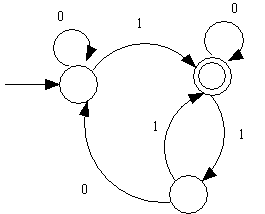
\includegraphics[width=7cm]{c1.png}
   \caption{Hand designed DFA}
   \label{Fig:dfa1}
\end{figure}

\begin{figure}[htbp]
   \centering
   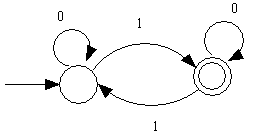
\includegraphics[width=7cm]{tb4.png}
   \caption{Corrected DFA}
   \label{Fig:dfa2}
\end{figure}

\subsection{Trakhtenbrot-Barzdin Algorithm}
Next I want the Trakhtenbrot-Barzdin (TB) algorithm to generate the same DFA by using the correct training data set. After playing around with the training set the following gave the correct DFA. See Question 2 for a description of the input format.
\begin{verbatim}
6 2
1 1 1
0 1 0
1 3 0 1 0
1 2 0 1
1 2 1 0
0 2 1 1
\end{verbatim}
Fig~\ref{Fig:tb1}-\ref{Fig:tb4} shows how the prefix-tree acceptor is merged to generate the correct DFA.

\begin{figure}[htbp]
   \centering
   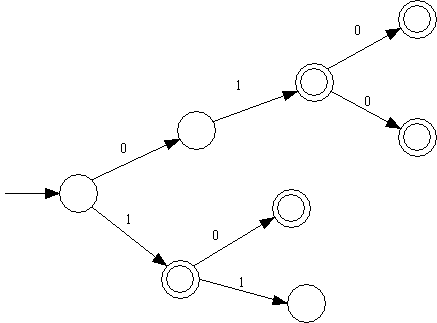
\includegraphics[width=7cm]{tb1.png}
   \caption{Step 1}
   \label{Fig:tb1}
\end{figure}

\begin{figure}[htbp]
   \centering
   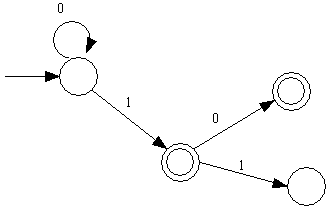
\includegraphics[width=7cm]{tb2.png}
   \caption{Step 2}
   \label{Fig:tb2}
\end{figure}

\begin{figure}[htbp]
   \centering
   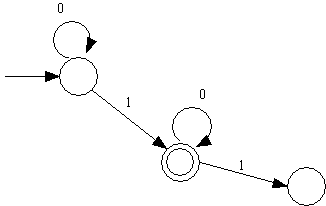
\includegraphics[width=7cm]{tb3.png}
   \caption{Step 3}
   \label{Fig:tb3}
\end{figure}

\begin{figure}[htbp]
   \centering
   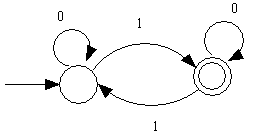
\includegraphics[width=7cm]{tb4.png}
   \caption{Step 4}
   \label{Fig:tb4}
\end{figure}

\section{Question 2}
The purpose of this question was to develop a evidence driven state merging algorithm for deterministic finite automata (DFAs). The algorithm that was chosen was the blue-fringe control strategy using grammar induction as described in \cite{lang}. The application was developed in Java 1.5.0 in Mandriva Linux 2006. The application can be executed by typing \emph{java blueFringe} in the console. This will display a list of possible parameters that can be passed to the application. The important parameter that needs to be passed is the name of the input training file. It is possible to also save the generated DFA to an output file. A image sequence of all the iterations of the algorithm can also be saved. This image sequence does not always display the DFA correctly, especially when a state transitions to itself. It was only added to help in the visualisation of the algorithm.

The training file's format have to be the same as the prefix-tree acceptor format. This is an example of a possible training file:

\begin{verbatim}
8 2
1 1 1
0 1 0
1 3 0 1 0
1 2 0 1
1 2 1 0
0 2 1 1
0 3 1 0 1
0 3 1 1 0
\end{verbatim}

The first line tells us how many possible inputs follow. This is followed by the size of the input language. This application only accepts input that has a language size of two. The rest of the lines are input strings that follow the following format,

$label$ $len$ $sym_1...sym_{len}$
\newline
, where \emph{label} is 0 when this input string rejects and 1 if it accepts. \emph{len} is the length of the input string. This is followed by the characters of the input string.

\subsection{Initial Configuration}
Before the algorithm can start iterating we need to do some initial setup. Firstly the training file should be loaded and the initial prefix tree created. Once this is done the initial colouring of the states should start. In the blue-fringe algorithm there are three types of colours. When a state is coloured red it means that the state can not be merged with any other red states. A blue state is the child of a red state and they are the states that are able to merge with a red state. The rest of the states in the DFA are coloured white.

For the initial configuration the root state is coloured red and his children coloured blue. The rest of the states are coloured white. The initial configuration of the above training file can be seen in Fig.~\ref{Fig:step1}.We are now able to move on to the actual algorithm.

\begin{figure}[htbp]
   \centering
   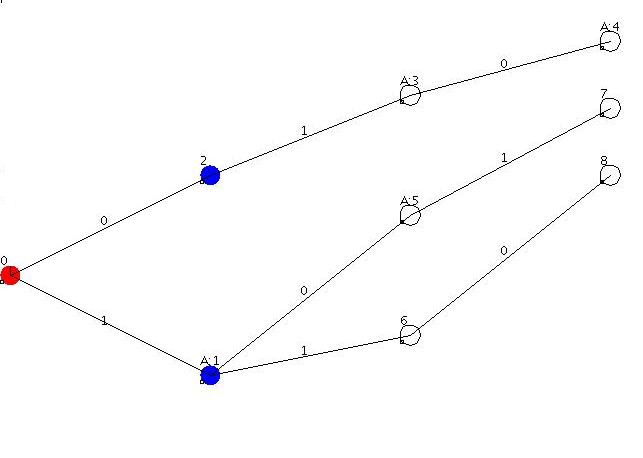
\includegraphics[width=10cm]{step1.png}
   \caption{Initial Configuration}
   \label{Fig:step1}
\end{figure}

\subsection{Blue-Fringe Algorithm}
The blue-fringe algorithm as I implemented it works as follows. When necessary the steps will be discussed in the subsequent subsections.
\begin{verbatim}
Step 1. Evaluate all possible red and blue state merges
Step 2. Do the red blue merge with the highest score.
        Go to Step 1.
Step 3. If there are no blue states that can merge with red states.
        Colour them all red and their children blue.
        Go to Step 1.
Step 4. If all states are coloured red.
        Stop.
\end{verbatim}
\subsubsection{Step 1}
Merges between red and blue states are evaluated by traversing the DFA and finding the amount of transitions they share. These transitions are only acceptable if every possible transition is the same. If one state has a transition that the other doesn't have this is ignored. The score of the possible merge that is returned is the amount of transitions that they share. If any transition failed a score of -1 is returned.
\subsubsection{Step 2}
Merging is done by taking a blue state and traversing it while simultaneously traversing the red state. If it is found that the blue state contains transitions that the red state does not have the transitions is added. When this is done all the states that had transitions to the blue state is changed to transition to the red state.
\subsection{Testing}
To test my implementation of the blue-fringe algorithm I decided to try to generate the DFA from Question 1. I used the prefix-tree acceptor I designed to create the DFA. This data led to the wrong DFA every time. It did however with the help of the image sequences make it easier to find errors in my application. After many tries I finally found a string (01) that should accept that I did not include in my initial data set. When this string was added the DFA was generated in five iterations. What was very interesting was that this enabled me to use less strings for the prefix-tree to generate the DFA. The same was applicable for the Trakhtenbrot-Barzdin (TB) algorithm in Question 1.

When my application generated the DFA the following output was generated when debug output was turned on,
\begin{verbatim}
java blueFringe -i a -t test -o output.txt -d

Loading training data
There is 8 items
Doing initial node coloring

Writing image
a0.jpeg written...
blue:2, red:0
score: 2
best score: 2
Best scoring states:2 and 0
Merging 2 and 0
Writing image
a1.jpeg written...

best score: -1
Promoting all blues
Writing image
a2.jpeg written...

blue:6, red:0
score: 1
blue:5, red:1
score: 1
best score: 1
Best scoring states:6 and 0
Merging 6 and 0
Writing image
a3.jpeg written...

blue:5, red:1
score: 1
best score: 1
Best scoring states:5 and 1
Merging 5 and 1
Writing image
a4.jpeg written...

best score: -1
DFA created
Writing dfa file
2 2
0 0 0 1
1 1 1 0
\end{verbatim}
\subsection{Summary}
When the DFA from Question 1 was tested I found that this algorithm was very effective. The TB algorithm obtained the correct DFA in four steps compared to the five of the blue-fringe algorithm. Although this is worse it is not a problem. The reason for this is that the blue-fringe algorithm is designed for generating DFAs that are much more complex than this example. The TB algorithm should technically always beat the blue-fringe algorithm on simple DFAs because the blue-fringe algorithm is an extension of the TB algorithm designed for generating more complex DFAs as was discussed in \cite{lang}.

I did compare the time it takes for both algorithms to generate the DFA. The TB algorithm was faster but I decided to ignore this fact because they were not both developed in the same programming language. The reason I decided on this is because my application executes inside the Java environment which is much slower than a native C application.
\section{Question 3}
For this question I added the ability to detect noise in an input file to the application developed in Question 2. To execute this program type \emph{java blueNoise} in the console to execute it. A list of possible parameters will be given.

This application makes the assumption that every training file contains noise. To determine which strings contain noise the following algorithm is followed. One string is removed from the training file and a DFA is generated. The string that has been remove is then tested on this DFA by using the score function. This process is repeated for every string in the training set. All strings that gave a negative score is then removed from the training set. This new training set is then used to build a DFA. I tested this on the training data from the previous example and although the correct DFA was not found the result was very close.

\begin{thebibliography}{9}
\bibitem{lang} K. Lange, A. Pearlmutter, A. Price
\emph{Results of the Abbadingo One DFA Learning
Competition and a New Evidence-Driven
State Merging Algorithm}


\end{thebibliography}
\end{document}
